% Compile from the repository root; see README.md in this directory.
\documentclass[tikz,border=8pt]{standalone}
\usepackage{fontspec}
\setmainfont{lmsans10-regular.otf}[BoldFont=lmsans10-bold.otf]
\usetikzlibrary{arrows.meta,positioning,calc}
\ifdefined\AMRDarkTheme
  \definecolor{ink}{HTML}{E6EDF3}
  \definecolor{blueFill}{HTML}{1C2D42}
  \definecolor{greenFill}{HTML}{1D3228}
  \definecolor{lavenderFill}{HTML}{302941}
  \definecolor{loopBlue}{HTML}{79C0FF}
  \definecolor{stopAmber}{HTML}{E3B341}
\else
\definecolor{ink}{HTML}{25354A}
\definecolor{blueFill}{HTML}{E7F0FB}
\definecolor{greenFill}{HTML}{E9F4ED}
\definecolor{lavenderFill}{HTML}{EFEDF8}
\definecolor{loopBlue}{HTML}{28649C}
\definecolor{stopAmber}{HTML}{94602C}
\fi
\tikzset{
  stage/.style={rounded corners=5pt,draw=ink,line width=1.1pt,
    fill=blueFill,text=ink,align=center,text width=6.4cm,
    minimum height=1.35cm,inner xsep=7pt,inner ysep=8pt},
  flow/.style={-{Latex[length=2.8mm,width=2mm]},draw=ink,line width=1.15pt},
  feedback/.style={draw=loopBlue,line width=1.05pt},
  stop/.style={draw=stopAmber,line width=1.05pt,dashed},
  note/.style={align=center,text width=2.5cm,font=\fontsize{12}{15}\selectfont}
}
\begin{document}
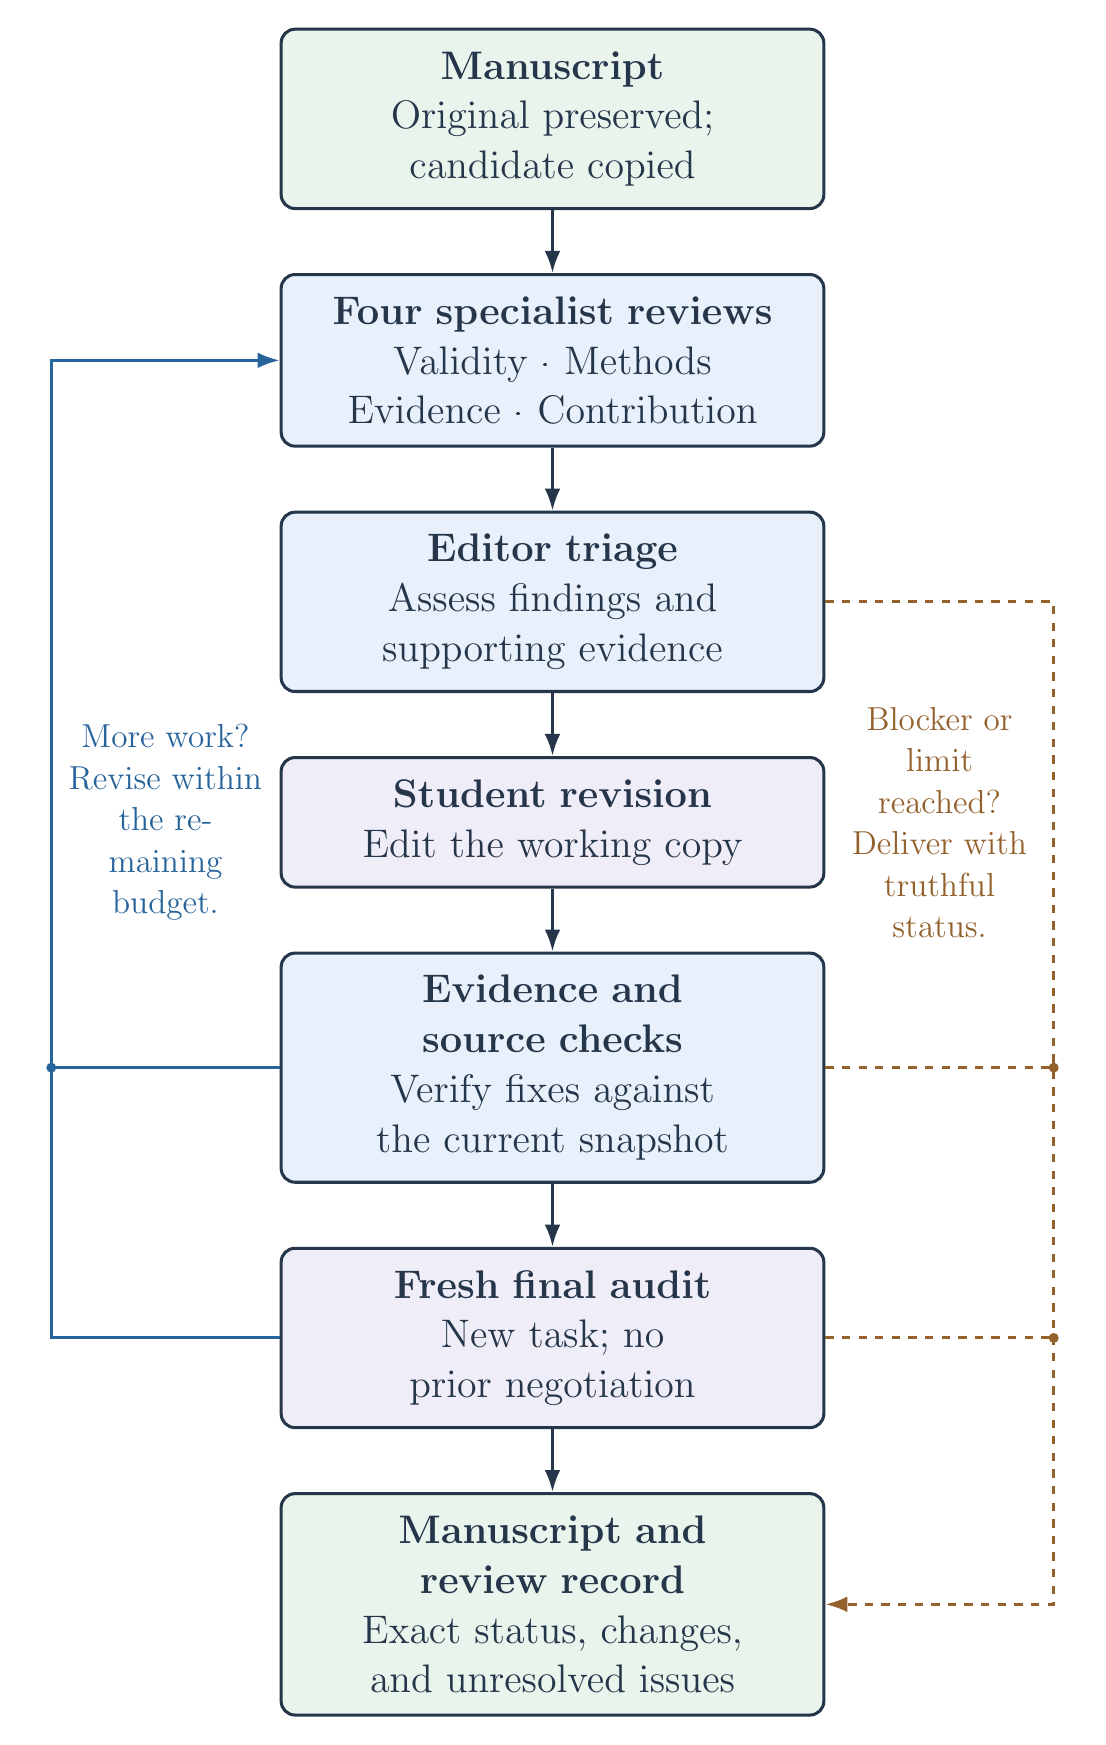
\begin{tikzpicture}[font=\fontsize{14}{18}\selectfont,node distance=8mm]
  \node[stage,fill=greenFill] (input)
    {\textbf{Manuscript}\\Original preserved; candidate copied};
  \node[stage,below=of input] (reviews)
    {\textbf{Four specialist reviews}\\Validity · Methods\\Evidence · Contribution};
  \node[stage,below=of reviews] (editor)
    {\textbf{Editor triage}\\Assess findings and supporting evidence};
  \node[stage,fill=lavenderFill,below=of editor] (student)
    {\textbf{Student revision}\\Edit the working copy};
  \node[stage,below=of student] (checks)
    {\textbf{Evidence and source checks}\\Verify fixes against the current snapshot};
  \node[stage,fill=lavenderFill,below=of checks] (audit)
    {\textbf{Fresh final audit}\\New task; no prior negotiation};
  \node[stage,fill=greenFill,below=of audit] (delivery)
    {\textbf{Manuscript and review record}\\Exact status, changes, and unresolved issues};

  \foreach \a/\b in {input/reviews,reviews/editor,editor/student,
    student/checks,checks/audit,audit/delivery}
    \draw[flow] (\a.south) -- (\b.north);

  % Shared feedback lane: explicit junction for checks and final-audit findings.
  \coordinate (reviewLane) at ($(reviews.west)+(-2.9cm,0)$);
  \coordinate (checkLane) at (reviewLane |- checks.west);
  \coordinate (auditLane) at (reviewLane |- audit.west);
  \draw[feedback,-{Latex[length=2.8mm,width=2mm]}]
    (audit.west) -- (auditLane) -- (reviewLane) -- (reviews.west);
  \draw[feedback] (checks.west) -- (checkLane);
  \fill[loopBlue] (checkLane) circle (1.8pt);
  \node[note,text=loopBlue] at ($(student.west)+(-1.45cm,0)$)
    {More work?\\Revise within\\the remaining\\budget.};

  % A separate termination lane reaches delivery without implying acceptance.
  \coordinate (stopTop) at ($(editor.east)+(2.9cm,0)$);
  \coordinate (stopCheck) at (stopTop |- checks.east);
  \coordinate (stopAudit) at (stopTop |- audit.east);
  \coordinate (stopBottom) at (stopTop |- delivery.east);
  \draw[stop,-{Latex[length=2.8mm,width=2mm]}]
    (editor.east) -- (stopTop) -- (stopBottom) -- (delivery.east);
  \draw[stop] (checks.east) -- (stopCheck);
  \draw[stop] (audit.east) -- (stopAudit);
  \fill[stopAmber] (stopCheck) circle (1.8pt);
  \fill[stopAmber] (stopAudit) circle (1.8pt);
  \node[note,text=stopAmber] at ($(student.east)+(1.45cm,0)$)
    {Blocker or\\limit reached?\\Deliver with\\truthful status.};

  % Explicit symmetric bounds keep the vertical spine centered in the README.
  \coordinate (leftGuard) at ($(reviewLane)+(-3mm,0)$);
  \coordinate (rightGuard) at ($(stopTop)+(3mm,0)$);
  \path[use as bounding box] (leftGuard |- input.north)
    rectangle (rightGuard |- delivery.south);
\end{tikzpicture}
\end{document}
